\section{Problem Analyzation}\label{problem}
    %ADD TABLES TO EACH SECTION TO PRESENT THE PROBLEMS MORE DIRECTLY
    In this paper, we focus on developing a general platform for eczema diagnosis. The development process can be divided into three parts, data, model and software, each part can be further divided into specific task. The more detailed methodologies toward tasks will be further explained in section \ref{Approaches}.
    \begin{Figure}
        \centering
        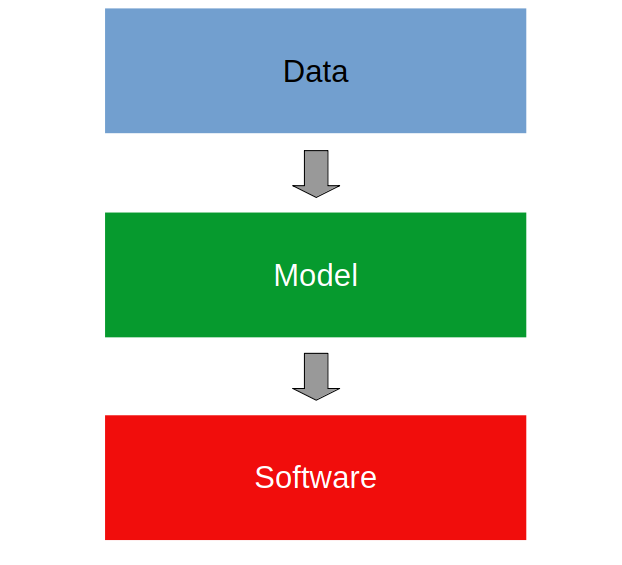
\includegraphics[width=\linewidth]{Image/WorkFlow.png}
        \captionof{figure}{General development workflow}
    \end{Figure}
    \subsection{Data}
        Data is one of the most important parts in making machine learning model. In building of eczema model, we would need as much high-quality data as possible. To be more specific, we need to create a dataset with label and low noise. There are mainly two process in data, collection and augmentation. There is survey shows that data scientists spend more than 65\% of their time into processing data\cite{AnacondaSurvey}.
        \begin{Figure}
            \centering
            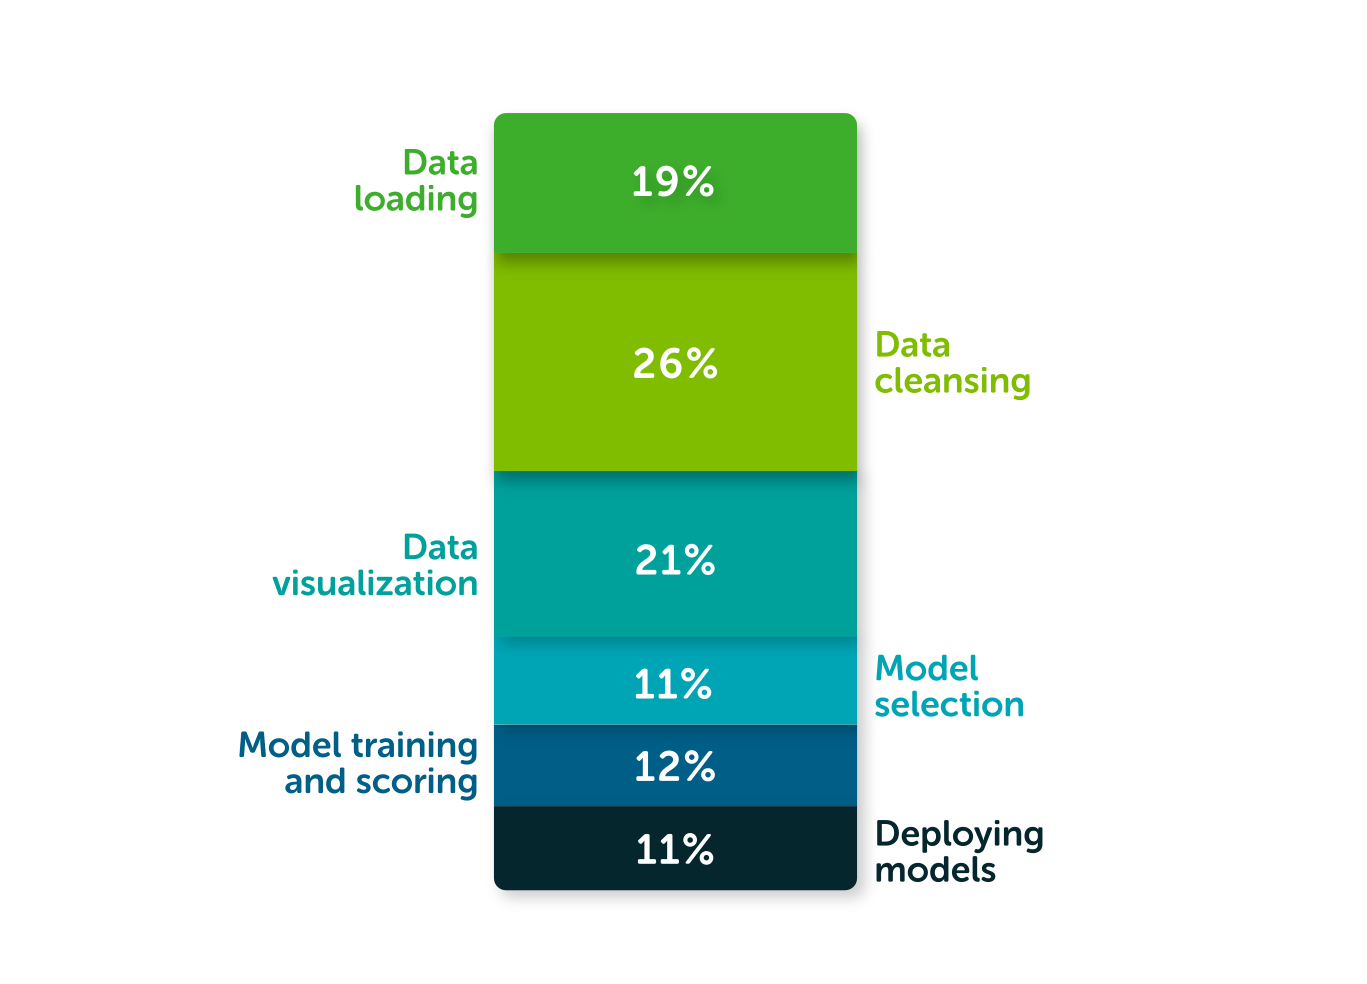
\includegraphics[width=\linewidth]{Image/Stacked-Chart.png}
            \captionof{figure}{A survey result from Anaconda in 2020\cite{AnacondaSurvey}}
        \end{Figure}
            \subsubsection{Data collection}
                A high-quality dataset can largely reduce the difficulty in model training. Therefore, data collection would be a crucial part in the development of our proposed platform. There are mainly two method of data collection, from internet and from ourselves.

                Considered the limited resources we have, building up our own first-hand dataset seems to be unrealistic since it required massive invest in collecting raw data from patient and possibly collaborate with clinic dermatologists to label the data. Therefore, collecting exist data from internet is a more appropriate choice, the paper would focus on this channel as well.

                The data we need to collect would variate based on the target feature and model used. Generally, we would need labeled digital image data of different eczema subtype, including asteatotic dermatitis, atopic dermatitis, contact dermatitis, dyshidrotic eczema, neurodermatitis, nummular dermatitis, seborrheic dermatitis, stasis dermatitis and subacute eczema, in total nine types of eczema. Theoretically, the images should only consist the affected part of eczema with plain background to minimize the noise in data for an accurate model, however, a collection of such data would be difficult. In addition, considered the label of eczema data would need talents with professional education in dermatology, self-label would not be appropriate in our case.

                Notice that we might not only need data in eczema, some methodologies may require other data for model pre-training. Therefore, we might need data of other skin diseases as well.

                Moreover, the distribution between different subtypes should be as balance as possible, since unbalance dataset would lead to decrease in models' generalizability. The diversity of data should also be considered as model may overfit into one specific kind of data, like eczema on white people, and thus cause worse performance in other kind of data.

                In conclusion, the main problem in data collection are:
                \begin{enumerate}
                    \item Collect sufficient data
                    \item Ensure the quality of collected data
                \end{enumerate}

            \subsubsection{Data augmentation}

                Data augmentation is another important task in preparing data, especially when the collected data is insufficient and low quality. With low quality data, it is impossible to train out a nice model. Therefore, the data augmentation work would be the 

                In machine learning data augmentation work play a pivotal role in increasing the robustness, generalizability and interpretability of model. The task would involve multiple aspect, including expanding the dataset through operation like flipping, rotation and cutting to prevent overfitting in model training. The main idea of data augmentation work is to improve the quality of existing dataset, which means to make the data have less noise and more diverse.
                
                Usually, data augmentation work can be done automatically by designed program, but the need of manual feature extracting or data filtering is also possible.

                For our case, a medical purpose platform have high requirement on generalizability and robustness, therefore the data augmentation work became critical. Furthermore, since some subtype of eczema would have significantly fewer data than other subtypes, the balance between different subtypes would also be challenging for our model building. Therefore, data augmentation work that focus one balancing the dataset would also be needed.

                To sum up, The main focus in data augmentation part is:
                \begin{enumerate}
                    \item Improve the quality of dataset.
                    \item Data cleaning.
                    \item Transformation of data
                \end{enumerate}

        \begin{Figure}
            \centering
            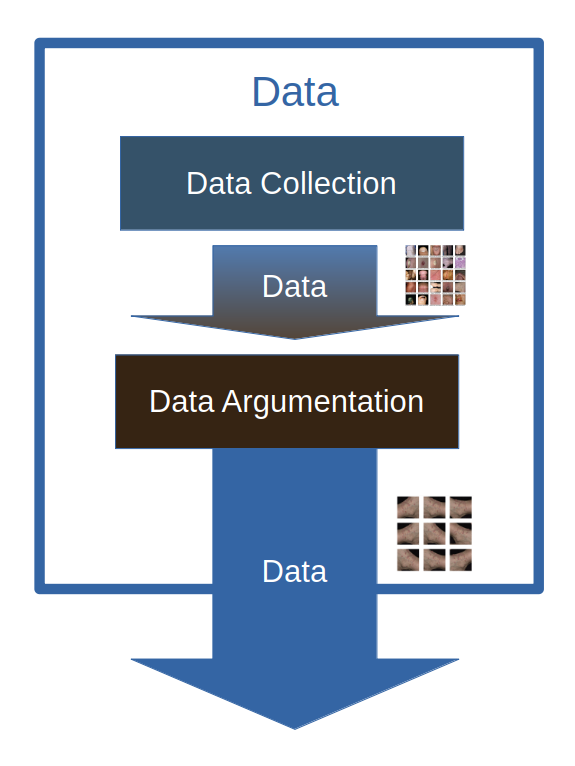
\includegraphics[width=\linewidth]{Image/DataWorkflow.png}
            \captionof{figure}{Workflow in data stage}
        \end{Figure}
    \subsection{Model}
        As the core part of our platform, model is the most important and also the most challenging part of our development. Considered our proposed platform would need to achieve not only one specific task in eczema diagnosis, but the whole process of diagnosis, we would need more than one model achieve that. A model for diagnosis the present of eczema on user, could use word input or image input or both. A model use to classify the eczema subtype, use image as input. A model provide personalized suggestion, based on the result from previous models. In each model development, there is also three stages, including model designing, model training and model evaluation.

        The workflow in model stage is not that straightforward like the one in data stage, which means it would not be step-by-step. The whole stage is recurrent and repeating, designed model may be trained and evaluated and then go back to designing for improvement.
        
        \begin{Figure}
            \centering
            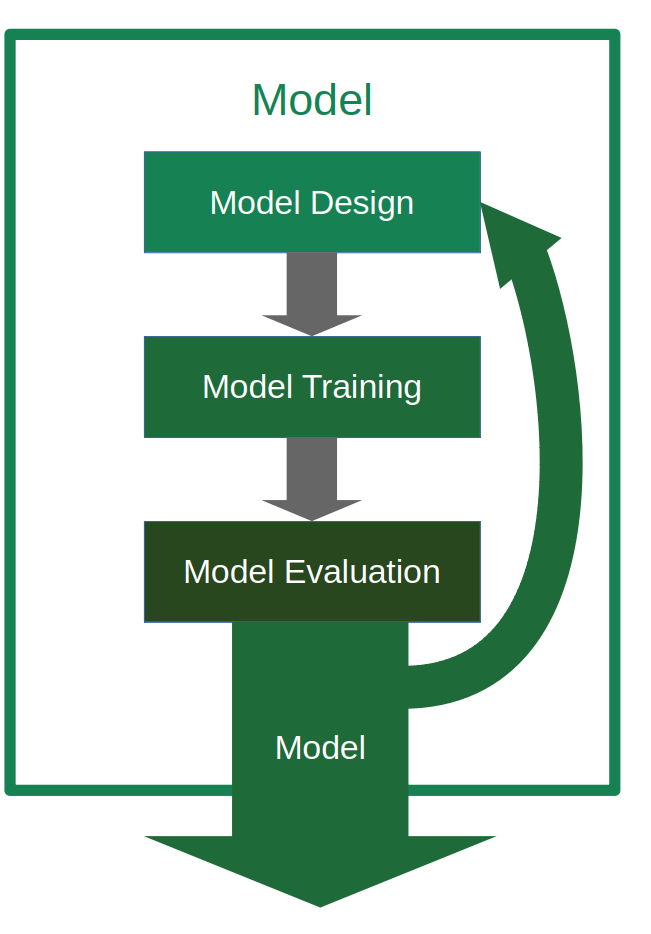
\includegraphics[width=\linewidth]{Image/ModelWorkflow.png}
            \captionof{figure}{Workflow of model stage}
        \end{Figure}

        \subsubsection{Model design}
            In machine learning, there are plentiful of different algorithm and architecture that can build up a model. Different architecture have their own advantages and disadvantages. Choosing an appropriate structure is crucial.

            Designing model structure needs to considered different factors and requirement toward the model. For instance, when designing model for image classification, models like convolutional neural networks may have better performance. Furthermore, design of models leads to the efficiency of model. When designing models for edges, lighter model with fewer parameters would be preferred.

            Unfortunately, many models structure have very poor interpretability due to the high complexity, especially in deep learning networks. These models may have well performance for no reason. Therefore, trails on testing different model structure would be necessary to figure out the right model to use, which means we would need to try out different structures on same task to have a comparison between models for finding out the best approaches.

            In addition, some Hyperparameter optimization(HPO) work would be involved in this step as well, including decisions like number of layer, activation functions and optimization functions.

            In conclusion, the major focuses on this stage are:
            \begin{enumerate}
                \item Select model architectures based on different requirement.
                \item Change architectures based on the performance of model.
                \item Optimize macro hyperparameters.
            \end{enumerate}
        
        \subsubsection{Model training}
            After design of the model finished, the next step is model training. In this step, there are mainly two tasks, hardware preparation and HPO.

            GPUs have been the main method for machine learning training nowadays. Having enough computational resources is critical in machine learning project, with insufficient computational resources, training of model would never be possible. Considered we might have a large size model, training on multiple GPUs seems to be necessary. However, due to the limited resources, set up a multi-GPUs server for our training may not be possible. Therefore, the training would need to take place in multiple machines, so the bandwidth of networks, which decide the communication speed between machines, became critical. The setup of the whole training system could be complicated and time-consuming.

            HPO is another part of model training, a well HPO can increase more than 10\% model accuracy. In training stage, HPO mainly focus on parameters like learning rate. These parameters might not play such a crucial role like what model structure does, but it is still important for ensuring the performance of model.

            To sum up, the main tasks in model training are:
            \begin{enumerate}
                \item Set up training server with multiple GPUs.
                \item Ensure the performance of multi-machine training.
                \item Split the model into pieces to train on different machine.
                \item Optimize training-related hyperparameters.
            \end{enumerate}

        \subsubsection{Model evaluation}
            As the last part of model development, model evaluation provides an overview to models' performance. Based on the evaluation, we can decide whether the model is suitable for deployment or it still needs further improvement.

            There are many benchmarks that evaluate a model from different aspect, for example, accuracy and generalizability. Choosing the right evaluation method can reveal the actual performance of model.

            To sum up, the main tasks in model evaluation are:
            \begin{enumerate}
                \item Choosing appropriate benchmarks for evaluation
                \item Perform evaluation toward the models.
            \end{enumerate}
    \subsection{Software}
        The last stage of development would be software. In our proposed platform, we would need to develop a cross-platform application that integrate models and relevant eczema information for users. During this stage, we need to deploy the trained model into application, and develop a cross-platform software.

                
        \begin{Figure}
            \centering
            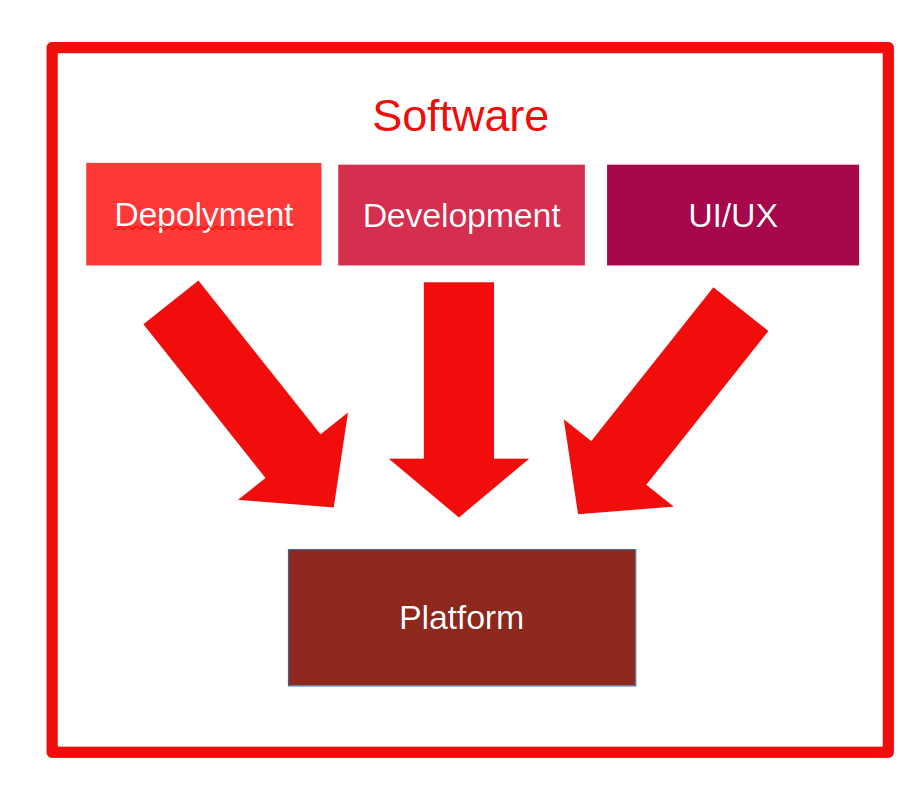
\includegraphics[width=\linewidth]{Image/SoftwareWorkflow.png}
            \captionof{figure}{Workflow of software stage}
        \end{Figure}

        \subsubsection{Model deployment}
            After training an up to standard model, the next step would be deploying the model into application.

            The main issue we need to concern is the efficiency of the model. If the model required too much computational resources or have exceeded model size, deployment into edges like iOS and Android is impossible. To cope with that, we need to either be aware of the model size at the designing stage or use other method like model distillation to reduce model size and complexity.

            Furthermore, the performance of model after deployment should be tested as well to ensure the performance under production environment consist with performance under development environment. 

            In conclusion, problems in model deployment are:
            \begin{enumerate}
                \item Deployment of model into software.
                \item Distillation of model to fit in devices (If needed).
            \end{enumerate}
        \subsubsection{Development}
            The development of software would be the main part of software. It decides the users' experience of our platform.
            
            To develop a cross-platform application, we would need to use some framework to reduce the workload. However, the development of application still required a large amount of code and effort. The main features of our platform are:
            \begin{enumerate}
                \item Automatic eczema diagnosis (diagnosis \& classification).
                \item Give personalized suggestion to users.
                \item Provide information about eczema.
            \end{enumerate}
            While the major part of first two features have been done in the model building stage, we still need to work on it in development stage as an interface for user to actually use these features.

            For the last features, we need to collect reliable information about eczema. We could include information like basic knowledge about eczema, how to prevent eczema and the treatment of eczema.

            At last, we would need testing on software to ensure the performance of application in practice meet the standard.

            In conclusion, tasks in software development are:
            \begin{enumerate}
                \item Implement the designed features.
                \item Cross-platform development of the application.
                \item Testing the software.
            \end{enumerate}
        \subsubsection{UI/UX}
            User interface and experience (UI/UX) is another task in software development. A well-designed UI/UX can provide better experience.

            The UI/UX design for our proposed platform should be friendly to our users, who are mainly patients suffer from eczema. The design should be able to navigate users to the right place in the application. Furthermore, since the platform consist multiple models for different functions, it's crucial to ensure all models are easily accessible for users with different needed. For instance, access to the classification model should not require the use of diagnosis model before.

            The UI/UX design is still important in the software development to make the features of application accessible for all users.

            In conclusion, major difficulty in UI/UX are:
            \begin{enumerate}
                \item Design user-friendly UI for the application.
                \item Make sure the accessibility of features.
            \end{enumerate}